% proposal.tex
\documentclass[main.tex]{subfiles}
\begin{document}
\chapter{Proposed Work} \label{ch:proposal}


The use of AM technologies to produce small batches of highly customized, complex parts, in a reduced development cycle results extremely attractive. While constructing failure envelopes can help overcome the wariness of industrial segments to design end-user parts, this resource is still not easy to implement, requiring a large number of mechanical tests and specialized equipment to properly map the failure behavior of a particular material. Additional complexity stems from what was shown in Section \ref{sec:SSICAM}: processing the same material under related AM technologies yields completely different failure envelopes, implying that no generalizations should be made, and each material-process pairing needs to be studied on a case-by-case basis.

The solutions presented in this proposal are aimed at providing the tools required to understand and predict properties and mechanical performance of parts manufactured through FFF, although some, if not all of the procedures explained here can be extrapolated to other AM techniques. The end goal is having the framework necessary to streamline the development of failure envelopes for FFF as much as possible, making a compelling case for adoption of this technology in the production of end user parts subjected to complex loading conditions. Additional outcomes of this research will lead to the ability to model, monitor and control the process, and potentially help understand its underlying physics.

\begin{figure}[h]
	\center
	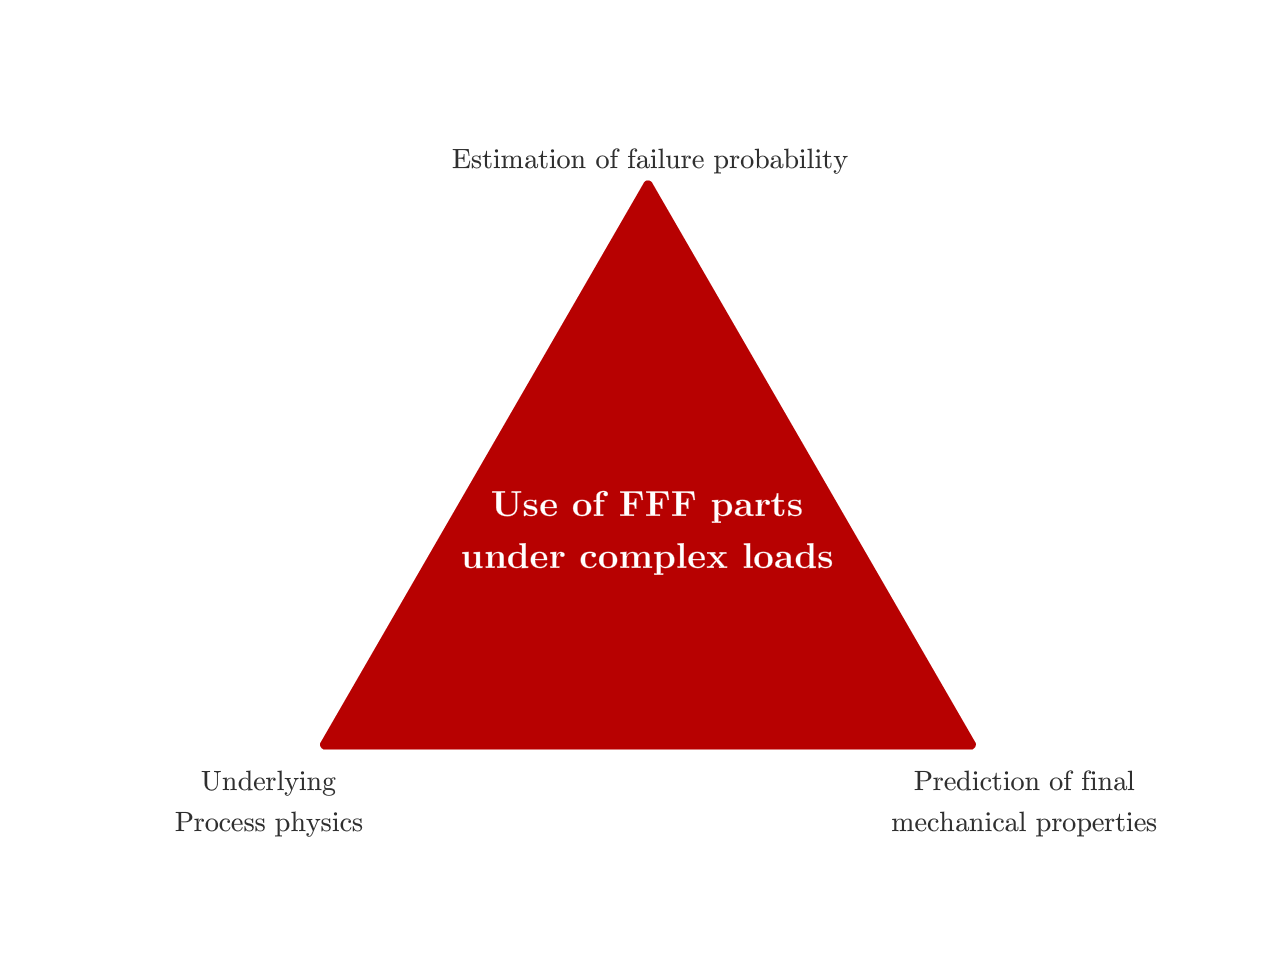
\includegraphics[height=7cm]{prelim_motivation}
	\caption{Different load directions in an anisotropic material} \label{fig:triangle}
\end{figure}
  

\section{Objectives} \label{sec:objectives}
\section{Preliminary results} \label{sec:prelim}
\section{Future work} \label{sec:fw}



%__________________________________________________________________________________________________________
% Nomenclature introduced in this chapter:
\nomenclature[A]{SSIC}{Stress-Stress Interaction Criterion}% 

% Symbols introduced in this chapter:
\nomenclature[S]{$X_t$}{Tensile strength in the 1-1 direction \nomunit{$MPa$}}
\end{document}